\section{The immune system and T cells}
The majority of metazoan organisms have an immune system, defined as a biological network of processes that defend the host organism against foreign pathogens and disease, that is vital for maintaining homeostasis. The earliest manifestation of an immune system first arose hundreds of millions of years ago in jawless fish in the form of variable lymphocyte receptors that recombined using a large panel of leucine-rich-receptors, creating the earliest lymphoid lineages \cite{Flajnik2010}. For mammalian immune systems, this biological network of processes is broadly broken into two major arms: the innate immune system and the adaptive immune system \cite{Dempsey2003}. The innate immune system initially responds to pathogens but is limited in the molecular scope of the threats it responds to, as it uses pathogen-associated molecular patterns (PAMPs) to trigger its activity, which are generally conserved. The innate immune system responds faster but generically to pathogens - which, while useful to the host for clearing the majority of infectious agents, means the innate immune system can be overwhelmed by pathogens that may have evolved to evade innate immune system processes \cite{Dempsey2003}. This set of circumstances creates the need for an adaptive immune system. 

\begin{figure}[htbp]
	\centering
	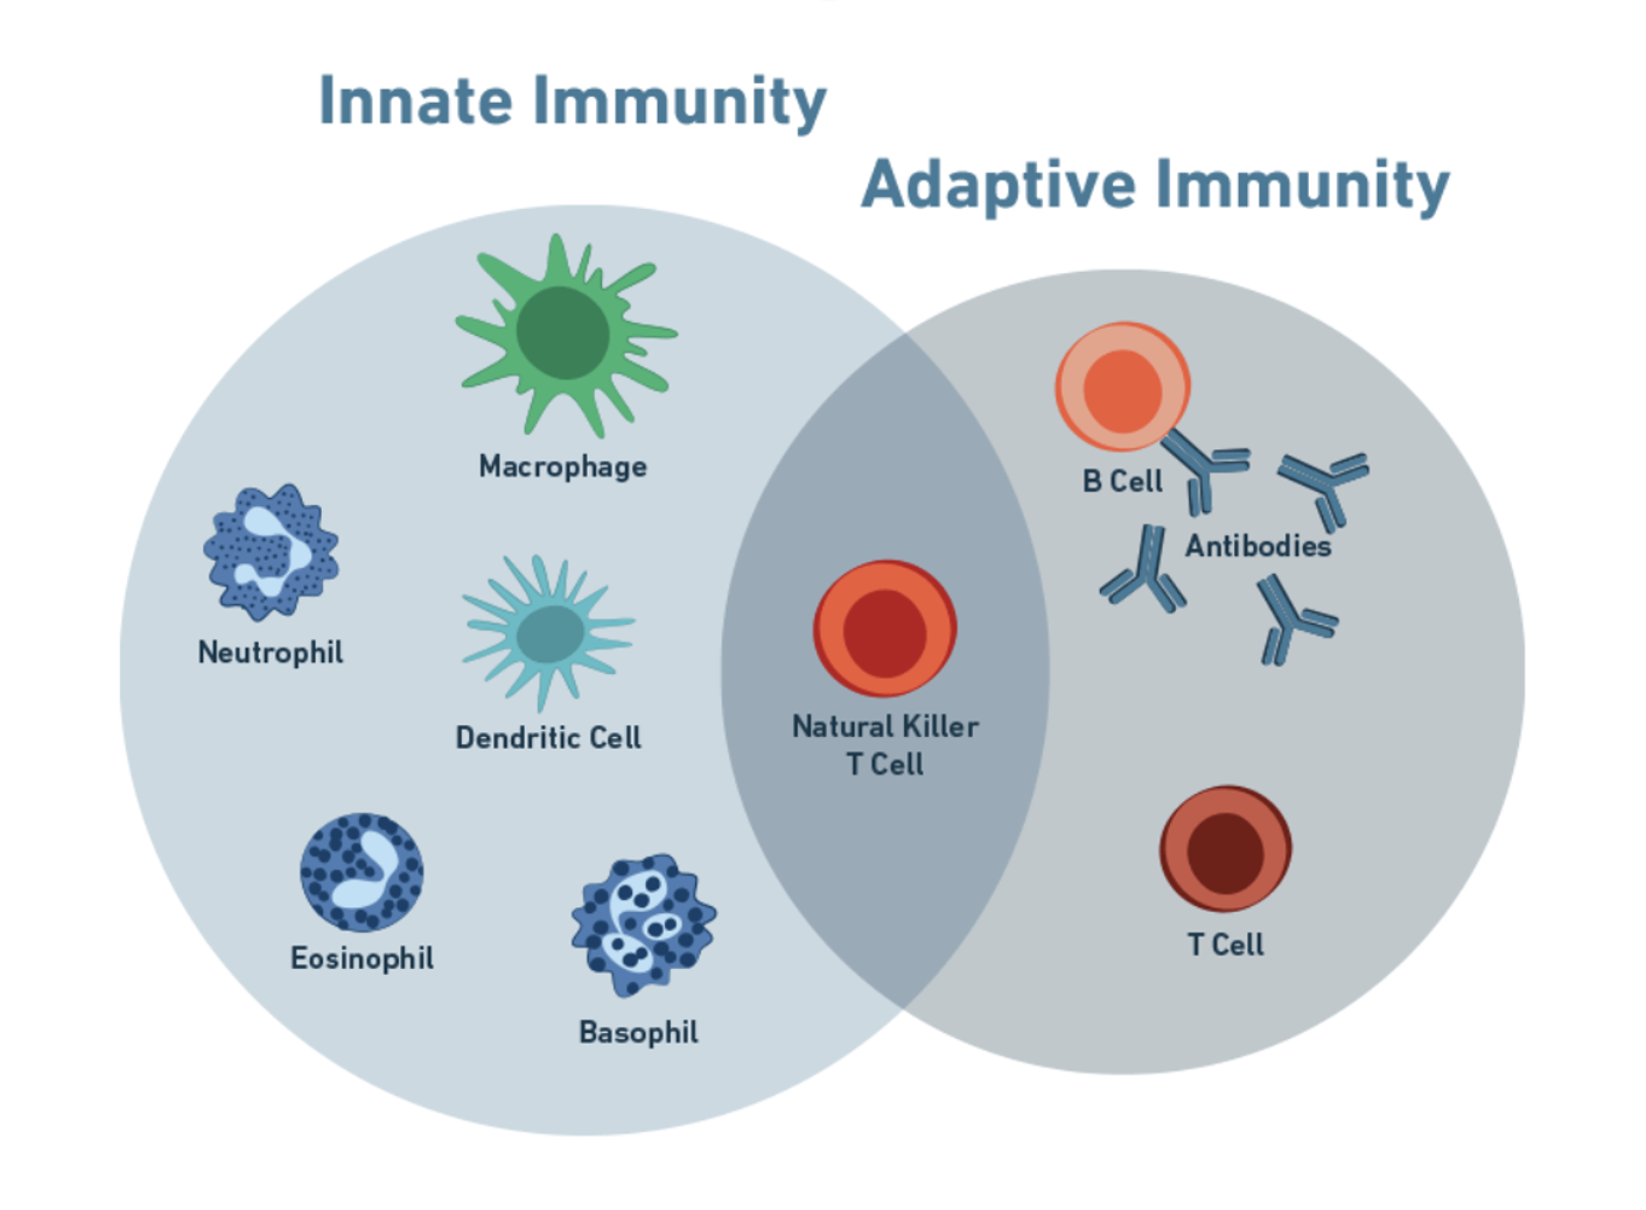
\includegraphics[width=\textwidth]{../figures/chapter1/innateadaptiveimmunesystem.png}
	\caption{Cell types of the innate vs. the adaptive immune system}
	\caption*{A schematic Venn diagram of the immune system. The typical conception of the vertebrate immune system is typically two-armed, broken into a faster-but-general responding innate immune system (left), and a slower-but-more-specific adaptive immune system (right), of which T cells are a part of. Almost all cell types that modern immunology research is concerned with falls somewhere within these two circles or their overlap - some immunology research is interested in characterizing certain effector or support immune cell types that fall in between innate and adaptive immunity (or can transfer their skills and interface between the two, calling into question the ontics of "innate" and "adaptive" immune systems) \cite{Heidegger1962}. This figure is adapted from \cite{Alam2007}.}
	\label{fig:innateadaptiveimmunesystem}
\end{figure}

The adaptive immune system responds much more slowly than the innate immune system, using this time to harvest and collect antigen and begin upramping of its antigen-specific molecular processes. The adaptive immune system is composed of two major types of cells (also called lymphocytes): B cells/lymphocytes and T cells/lymphocytes. B cells (named for originating from the bursa of Fabricus, the avian lymphoid organ in which B cells were first discovered \cite{Cooper2015}) produce antibodies that specifically bind to antigens and identify their bound partners as foreign entities meant for destruction. T cells on the other hand (named for originating in the thymus) directly manage the cytotoxic activity of the adaptive immune system. 

\section{T cell development}
T cells are composed of two main functional subtypes: CD8+ killer T cells (the primary focus of this thesis and heretofore referred to as any of the following: cytotoxic T lymphocytes (CTLs), cytotoxic T cells, CD8+ T cells) and CD4+ helper T cells. T cells as a whole are defined by their expression of the T cell receptor (TCR), the receptor responsible for recognizing foreign antigenic peptide presented by the target cell via its Class I or Class II Major Histocompatibility Complex (MHC, or pMHC). The TCR is composed of one TCR-$\alpha$ chain and one TCR-$\beta$ chain that associate to form the TCR. The vast majority of T cells (95\%+) express the TCR-$\alpha$ and TCR-$\beta$ chains and are thus called $\alpha \beta$ T cells, while the remaining 5\% of T cells expressing TCR-$\gamma$ and TCR-$\delta$ are called $\gamma \delta$ T cells. The TCR alone is insufficient for fully activating the T cell and requires additional signaling molecules to achieve complete signal transduction. The TCR additionally associates with one CD3$\gamma$ chain, one CD3$\delta$ chain, which are each associated with a CD3$\epsilon$ chain. A final two CD3$\gamma$ chains bind to the TCR to form the TCR signaling complex \cite{Germain2002}. There are a number of additional co-receptors that bind (either directly or indirectly) to the TCR. The most relevant to $\alpha \beta$ T cells are the CD8 or CD4 co-receptors, which define the specificity of the $\alpha \beta$ T cell to the two different classes of MHC. CD8+ T cells bind to MHC Class I, while CD4+ T cells bind to MHC Class II. 

The ability of T cells to properly recognize and engage only with foreign antigen while ignoring self-peptides is tightly regulated and begins at a very early stage in immune system development. T cells derive from hematopoietic stem cells (HSCs) that originate in the bone marrow. HSCs ultimately differentiate into common lymphoid progenitor cells (CLPs), which migrate to the thymus to ultimately differentiate into natural killer (NK), B, or T cells. 

The process of differentiating into T cells is primarily motivated by the need to create a functional TCR that does not react to self-antigen but does react to foreign antigen. As TCRs are made up of alpha and beta chains that are evolved to react to a wide range of possible antigens that an organism may encounter in its lifespan, T cell differentiation occurs in a carefully regulated, stepwise manner that first begins with TCR-beta chain selection. T cells at this stage express an invariant pre-alpha chain called pre-T$\alpha$ that the varying beta chains (generated by VDJ recombination of the TCR-beta locus) attempt to form a stable binding partner with. Once an appropriate TCR-beta chain is identified as capable of stable binding to pre-T$\alpha$ the same process begins on the TCR-$\alpha$ chain against the now mature TCR-$\beta$ chain, generating a stable (but not necessarily functional) TCR.

Once a stable TCR heterodimer has been formed, the T cells must undergo a two-step process of selection in order to build a functional repertoire of TCRs, called positive and negative selection. Positive selection involves presenting the T cells with self-peptides on MHC with the selection criteria of being able to bind with this complex. T cells that cannot bind either MHC Class I or Class II via their TCR do not receive survival signals and will die. This is called "death by neglect" - the removal of cells with TCRs that are unable to bind MHC (which is functionally useless to the organism). Therefore, the body positively filters/selects for T cells with TCRs that can recognize MHC molecules with moderate affinity, leaving those that cannot recognize MHCs to die off \cite{Palmer2003}.

\begin{figure}[htbp]
	\centering
	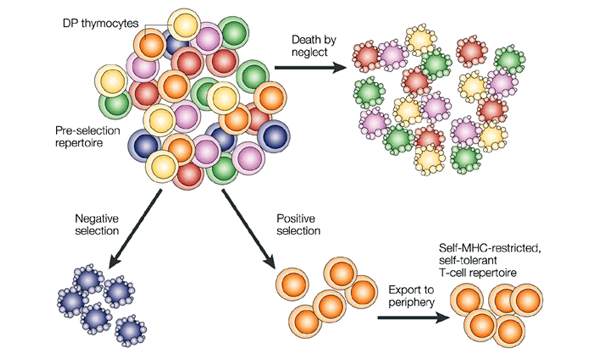
\includegraphics[width=\textwidth]{../figures/chapter1/posnegsel.png}
	\caption{Positive and negative selection}
	\caption*{Thymocytes that are double positive (DP) for CD4+ and CD8+ begin with an unselected repertoire of TCRs. The process of positive selection ensures that DP thymocytes that do not bind MHC Class I or II die ("death by neglect"), while those that do bind MHC will receive a signal to survive. Negative selection filters out TCRs that are too reactive to self-antigen, which would be intolerable for a functioning immune system. These selection processes results in the generation of T cells that are self-MHC restricted, self-antigen tolerant T cells that are ready to fight potential infection. This figure is adapted from \cite{Palmer2003}.}
	\label{fig:posnegsel}
\end{figure}

After obtaining T cells that are capable of binding to MHC molecules, the next step is called negative selection, during which the immune system selects for T cells that do not react to self-antigen. In this stage of selection, T cells that bind to MHC presenting self-antigen of \textit{high} affinities receive an apoptotic signal that leads to cell death. This ensures that T cells are capable of distinguishing self from non-self and are tolerant of self-antigen. Negative selection therefore selects for T cells that do not react to self-peptide. The vast majority of thymocytes (98\%+) fail to pass positive and negative selection. Following positive and negative selection, the resulting T cell set can bind to any antigen (presumably belonging to any foreign pathogen) so long that the antigen is distinct from the body’s self-antigens. 

After these stages of T cell development, these T cells (called naïve T cells) then exit the thymus and begin to circulate in the host, where they will spend their time surveying the host for disease and foreign antigens.

\section{TCR activation and downstream signaling}
	\label{TCR activation and downstream signaling}
If a CD8+ T cell engages an infected cell presenting foreign peptide, the T cell will initiate a cascade of antigenic-specific intracellular signaling events. Upon ligation of the TCR to the pMHC complex, the CD3 proteins (CD3$\epsilon \gamma$ and CD3$\epsilon \delta$ heterodimers and a CD3$\zeta$ homodimer) bearing ITAMs (immunoreceptor tyrosine-based activation motifs) get phosphorylated by Lck. Upon phosphorylation, cytosolic signaling proteins can bind to phosphorylated ITAMs and propagate the signal from the triggered TCR further downstream into the T cell. CD3$\zeta$ contains three ITAMs, while CD3$\delta$, CD3 $\gamma$, and CD3$\epsilon$ all only contain one ITAM. The CD3 chains are needed as the cytosolic tails of the $\alpha$ and $\beta$ subunits of the TCR is extremely short and structurally do not support significant adaptor features for signal amplification molecules. This modularity also allows for an increased range of TCR signaling for fine-tuning key features of the T cell effector response (e.g. killing, proliferation, signaling, cytokine secretion) in response to a number of diverse inputs such as antigen strength, lifetime of interaction, and number of bound-TCRs at the IS.

\begin{figure}[htbp]
	\centering
	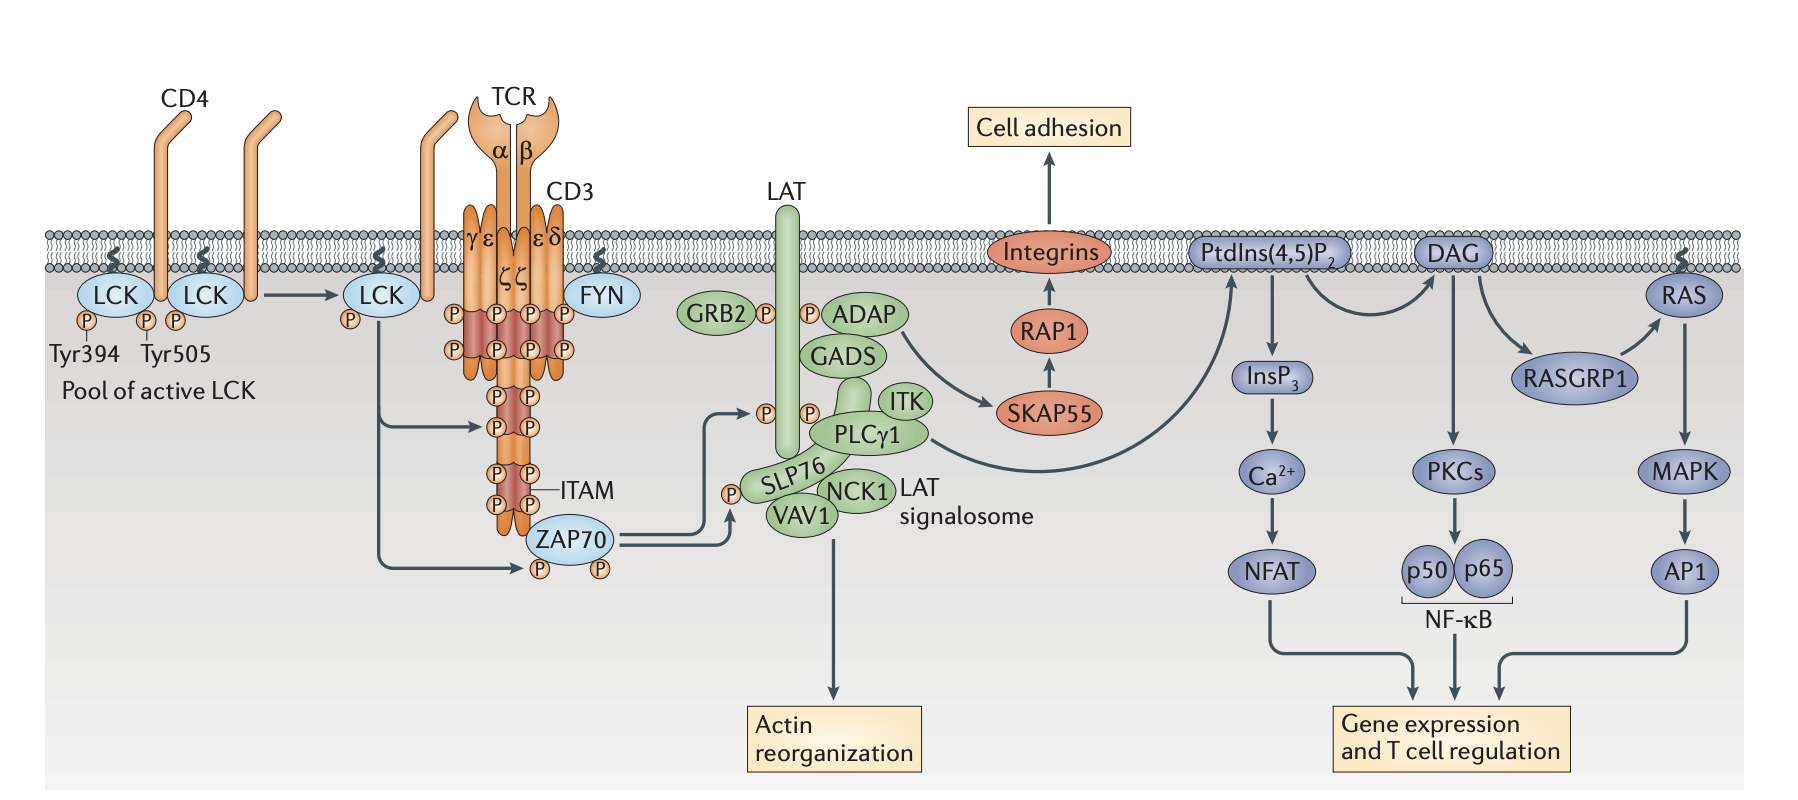
\includegraphics[width=\textwidth]{../figures/chapter1/tcrsignaling.png}
	\caption{The T cell receptor and its signaling partners}
	\caption*{An overview of TCR signalling. Signaling through the TCR commences upon recognition of cognate pMHC on the target surface. The assembly of the CD3$\gamma$, $\delta$, and $\zeta$-chains recruits Lck, which phosphorylates the ITAMs of the CD3$\gamma$, $\delta$, and$\zeta$ chains, recruiting ZAP70. Activated ZAP70 primes the LAT signalosome to coordinate critical signaling molecules such as PLC$\gamma$, GRB2, SLP76, ADAP, ITK, Nck1, and VAV1. The LAT signalosome is a node for three major signaling signaling pathways: the $Ca^{2+}$, the MAPK, and the NF-$\kappa$B pathway, which initiate critical signaling pathways for the expansion, differentiation, and activation of T cells. These signals also modify integrin signaling, which strongly influences cytoskeletal dynamics and adhesive and migratory behavior. The figure is adapted from \cite{Brownlie2013}.}
	\label{fig:tcrsignaling}
\end{figure}

The phosphorylated CD3 ITAMs recruit the protein tyrosine kinase ZAP70 that binds to the phoshorylated tyrosine motifs via its SH2 domains. This brings ZAP70 closer to CD8-bound Lck, which further phosphorylates ZAP70, activating ZAP70. Upon Lck-mediated phosphorylation of ZAP70, ZAP70 itself phosphorylates and activates the transmembrane protein called linker for activation of T cells (LAT). LAT acts as a scaffold, providing binding sites for a number of signaling molecules (via its own phosphorylated sites) that link these signaling molecules in space and time, including the SH2 domain containing leukocyte protein of 76 kDa (SLP76) which provides even further additional binding sites on the LAT signaling complex, SOS, GRB2, ITK, Vav, Nck1, and FYB (or ADAP).

One of the most crucial signaling molecules that binds to LAT is the protein phospholipase C$\gamma$1 (PLC$\gamma$), which generates key lipid secondary messenger molecules. Phosphatidylinositol 4,5-bisphosphate ($PIP_{2}$) is an input to PLC$\gamma$ function. Once phosphorylated and activated by Itk, PLC$\gamma$ uses $PIP_{2}$ as a substrate to enzymatically generate two products: diacylglycerol (DAG) and the soluble inositol 1,4,5-trisphosphate ($IP_{3}$). Diacylglycerol accumulates in the IS, which prompts recruitment of the microtubule motor protein dynein and drives polarization of the microtubule-organizing center (MTOC) \cite{Quann2009} and the recruitment of lytic granules to the immune synapse (this is further discussed in the T cell degranulation and target cell death introduction section, section \ref{T cell degranulation and target cell death} \cite{Stinchcombe2006}). $IP_{3}$ is soluble and diffuses throughout the cytosol, eventually binding to its receptor inositol trisphosphate receptor (InsP3R), located on the endoplasmic reticulum (ER). The binding of $IP_{3}$ to InsP3R triggers release of calcium ($Ca^{2+}$) ions from the ER into the cytosol, initiating calcium-dependent transcription programming. These include the NFAT, NF-$\kappa$B, and AP1 signaling pathways, all of which assist in fully activating the T cell. The depletion of calcium stores in the ER is detected by the Stormal interaction molecule 1 (STIM1) calcium sensor protein, and localizes to plasma membrane in puncta. Once STIM1 is near the plasma membrane, it activates the calcium channel Orai1 (Calcium release-activated calcium channel protein 1), which results in cytosolic calcium flux and further calcium-dependent gene expression \cite{Lunz2019}. This Orai1-mediated calcium flux is a required step for lymphocyte degranulation \cite{Maul-Pavicic2011}. Another notable lipid secondary messenger is phosphatidylinositol (3,4,5)-trisphosphate ($PIP_{3}$). $PIP_{2}$ is phosphorylated by the phosphoinositide 3-kinase (PI-3K) to give $PIP_{3}$, which further activates downstream signaling proteins, most notably Akt, which is highly involved in T cell metabolism.

The generation of spatial gradients and patterns of lipid secondary messenger molecules at the plasma membrane is highly consequential, resulting in the formation of a necessary killing and major signaling structure called the immunological synapse. 

\section{The immunological synapse and the T cell cytoskeleton}
\label{The immunological synapse and the T cell cytoskeleton}
The immunological synapse (also called the immune synapse) is the highly organized, structurally stereotyped interface that T cells form against an APC. It is classically characterized as a concentric, annular structure that bears a "bulls-eye" center surrounded by a ring of filamentous actin (see Figure \ref{fig:immunesynapse}a). The immune synapse is a major T cell signaling and killing megastructure, and robust formation of the immune synapse is essential for the T cell to achieve its maximal cytotoxic efficacy, in particular when concerned with lytic granule secretion (see \ref{T cell degranulation and target cell death}) \cite{Ritter2015}.

\begin{figure}[htbp]
	\centering
	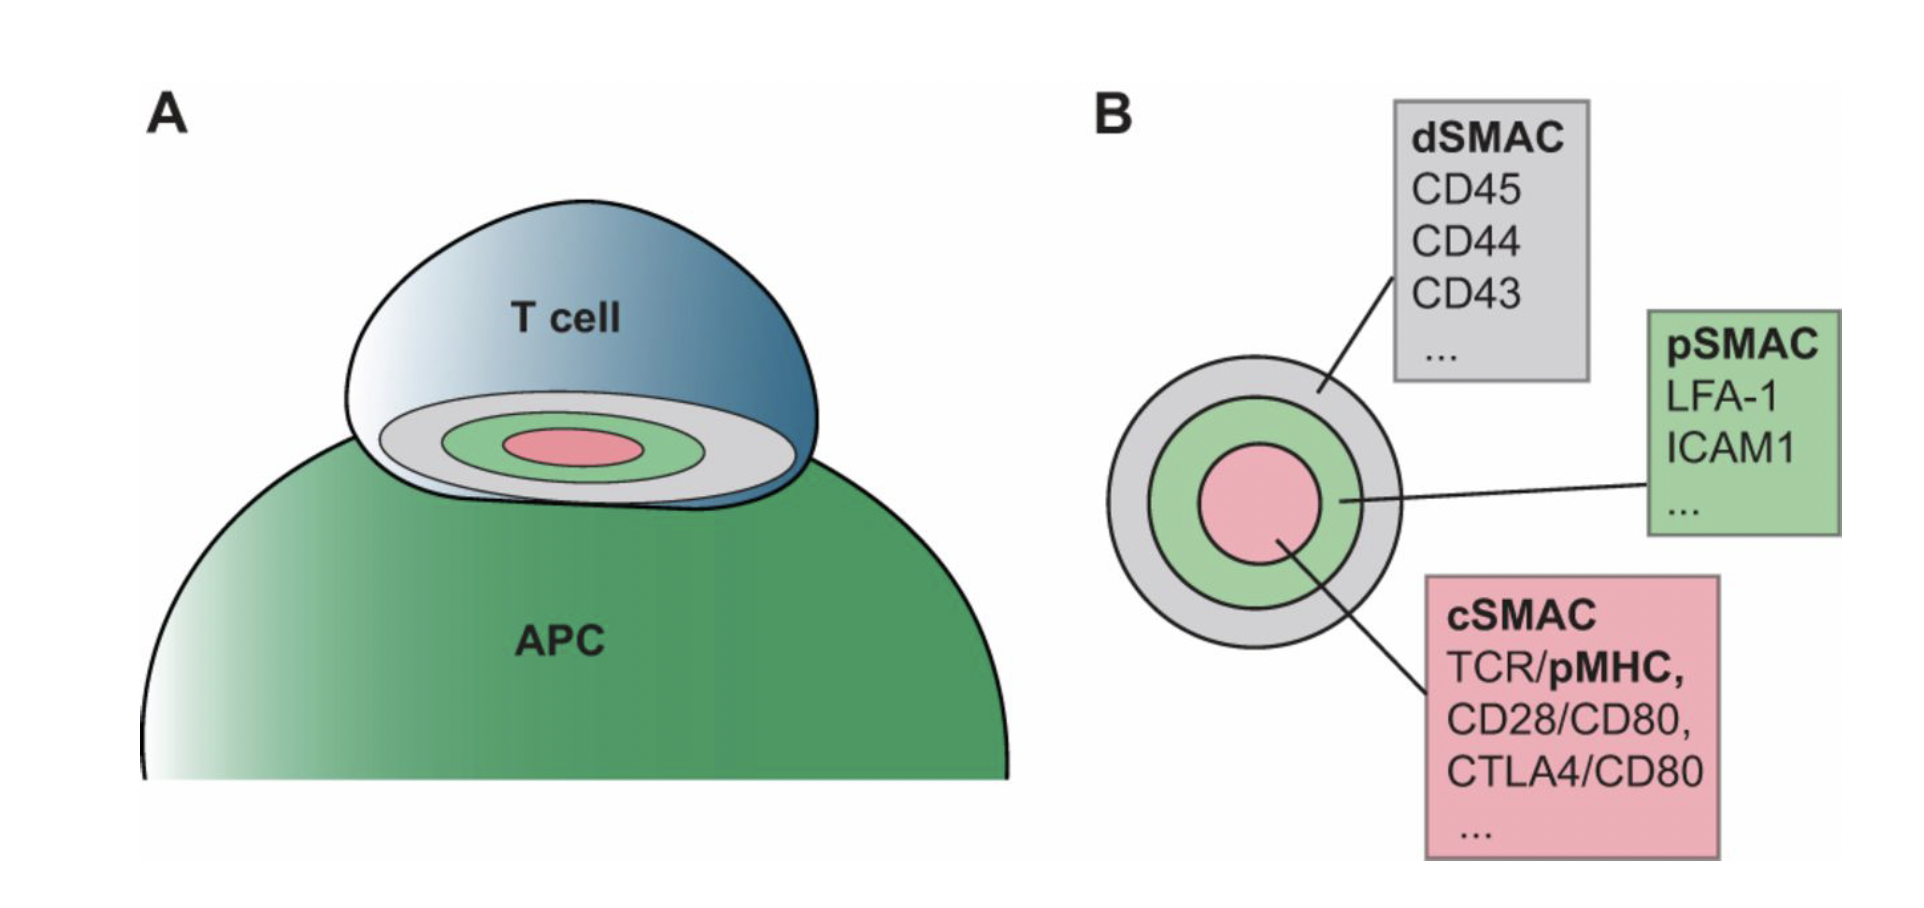
\includegraphics[width=\textwidth]{../figures/chapter1/immunesynapse.png}
	\caption{The immunological synapse}
	\caption*{\textbf{(A)}: A schematic of the canonical model of the immune synapse. The T cell (blue, above) is in contact with the APC (green, below). The IS is shown as a series of interfacial concentric rings. \textbf{(B)}: The IS is classically divided into three regions, extending from the center outwards: the cSMAC, the pSMAC, and the dSMAC. The proper formation of the IS results in functionally distinct and biochemically patterned regions. This figure is adapted from \cite{Yu2013}.}
	\label{fig:immunesynapse}
\end{figure}

Upon TCR activation, the actin cytoskeleton rapidly polymerizes and organizes itself to achieve an annular arrangement, forming the IS. Existing work in the field highlights the necessity of $PIP_3$ accumulation at the synapse for stepwise formation of actin structures \cite{LeFloch2013}. $PIP_3$ recruits the guanine exchange factor Dock2, which locally activates the Rho family GTPase Rac. This activated Rac then signals to the Wiskott-Aldrich syndrome protein family member 2 (WAVE2), generating lamellipodial growth \cite{LeFloch2013, Derivery2010}. Lipid gradients also control Cdc42, another Rho family GTPase. Together, $PIP_2$ and Cdc42 (activated by Vav1 \cite{Abe2000}) activate the Wiskott-Aldrich syndrome protein (WASP), generating filopodia \cite{KennethE.PrehodaJessicaA.ScottR.DycheMullins2000}.

WASP and WAVE2 are actin nucleation promoting factors that activate nucleation factors such as Arp2/3. Actin nucleation factors enable nucleation at sub-critical concentrations of g-actin \cite{Carlsson2005}. These proteins are essential for proper cytoskeletal remodeling, and the role of WASP and WAVE2 on immune synapse dynamics is the subject of Chapter \ref{chap:chapter2}, where their function proves to be critical for cytotoxicity.

From a macromolecular perspective, the IS is segregated into three supramolecular activation clusters (SMACs), called the central, distal, and peripheral supramolecular activation clusters (cSMAC, pSMAC, and dSMAC, respectively, and named in their order of concentricity starting from the center. See Figure \ref{fig:immunesynapse}b). The cSMAC contains the TCR signaling complex, CD28, and PKC$\theta$ \cite{Monks1998, Tseng2008}. The pSMAC contains the lymphocyte function-associated antigen 1 (LFA-1) and talin \cite{Monks1998}. The role of these proteins in lytic granule fusion and cytotoxicity is explored deeply in Chapter \ref{chap:chapter3}. Notably, the CD45 phosphotase is initially located in the pSMAC, but then is sterically excluded from the pSMAC due to its size to the dSMAC \cite{Johnson2000}. The dSMAC includes the filamentous-actin ring, as well as CD43 and CD44, proteins that are linked to adhesion and phenotypically dovetail with stronger T cell-target cell contact \cite{Yu2013}.

It is important to note that most of the work that has been done to investigate the "bulls-eye" model of protein localization in the immune synapse has been performed using lipid bilayer experimental systems with TIRF microscopy. However, this experimental approach neglects the 3D architecture of actual T cell-target cell contacts.  Approaches involving planar glass surfaces also fail to address significant amounts of evidence that immune synapses can take on additional organizations, such as TCR microvilli \cite{Kim2018} or multiple synapses against multiple targets \cite{Vorselen2020}. Other strategies have been developed to characterize immune synapses in more physically relevant environments \cite{Jin2019}, which should prove fruitful in truly understanding IS structure and dynamics.

Proper synapse formation (ranging widely from organization in space, organization in time, and presence/absence of certain molecular players) dramatically affects T cell cytotoxicity, which is discussed in following sections. This highlights the functional importance of the immune synapse.

\section{T cell degranulation and target cell death}
\label{T cell degranulation and target cell death}
The killing mechanism of CTLs is fundamental to robust anticancer and antiviral responses. CTLs achieve their cytotoxic effects by managing a two-pronged approach 1. specifically destroying only infected or oncogenic target cells (recognized via ligation between the TCR and its specific pMHC interaction) and 2. preserving the integrity of the surrounding healthy bystander tissue. Spatially, these aims are realized through the precise signaling mechanisms of the immune synapse.

The centrosome is a key determinant of lytic granule localization \cite{Stinchcombe2007, Huse2013}. Target cell recognition triggers the polarization of the centrosome to the immune synapse. Lytic granules containing the cytolytic proteins perforin and granzymes traffic along microtubules, placing them closer to the immune synapse for secretion. Sequential killing events involve rapid reorientation of the centrosome and microtubules to the adjacent membrane \cite{Kuhn2002}, demonstrating the centrosome's importance for lytic granule fusion at the synapse.

The subsequent secretion of the hydrophobic protein perforin and granzyme proteases from lytic granules through the immune synapse is the most prevalent mechanism of T cell-mediated killing of target cells \cite{Dustin2010, Stinchcombe2007} and is called \textit{degranulation}. When released, perforin oligomerizes in a calcium dependent manner \cite{Law2010} and forms pores on the target cell surface, (around 16nm in diameter) \cite{Cartwright2014}, inducing significant membrane damage. The target cell responds to this traumatic event at the plasma membrane using a mechanism that permits granzymes entry to the cytoplasm, where they cleave apoptotic substrates that induce apoptosis \cite{Keefe2005}. Because both infected and healthy cells are capable of being killed and cleared in this way, specialized mechanisms have evolved over time in immune cells to ensure that the effects of perforin and granzyme are constrained to the target cell alone.

Cytotoxic T lymphocytes store their perforin and granzymes in specialized secretory lysosomes called lytic granules (0.5 to 2 $\mu$m) \cite{Sanchez-Ruiz2011}, whose acidic pH environment quenches the lytic and apoptotic activity of both proteins \cite{Thiery2014, Keefe2005}. Following mere minutes of target cell recognition, the lytic granules are trafficked along microtubules to the immunological synapse (IS). At this site, they fuse with the plasma membrane, releasing their contents into the intercellular space.

\begin{figure}[htbp]
	\centering
	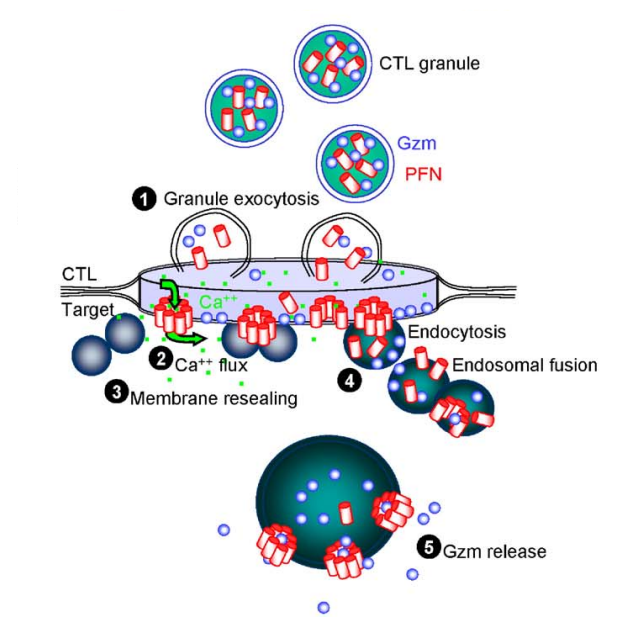
\includegraphics[width=\textwidth]{../figures/chapter1/degranulation.png}
	\caption{Lytic granule secretion and perforin pore formation}
	\caption*{A schematic of lytic granule secretion and entry of perforin and granzyme into the target cell. Lytic granules are coordinated to the immune synapse and selectively fuse at the synapse, emptying their cytotoxic contents, perforin (red) and granzymes (blue), into the intercellular space. Perforin requires the presence of calcium ions ($Ca^{2+}$, green) to pierce the target cell membrane. and permit entry of granzyme proteases. Target cell membrane repair programs begin to repair the damaged membrane.The resealing of the target membrane results in endocytosis of intercellular granzyme and perforin (as well as $Ca^{2+}$ ions), which again re-pierce the endocytic vesicular membrane and allow for true granzyme entry into the cytosol. where granzymes cleave apoptotic effectors. This figure is adapted from \cite{Keefe2005_2}.}
	\label{fig:degranulation}
\end{figure}

At the same time, F-actin and the associated actin nucleation promoting factors (NPFs) at the IS undergo significant spatiotemporal remodeling. This results in a highly complex landscape of highly dynamic actin sheets and protrusions \cite{Ritter2015}. Canonically, actin clearance from the center of the immune synapse (cSMAC) is required for fusion of lytic granules to the center of the synapse \cite{Ritter2015}. 

\begin{figure}[htbp]
	\centering
	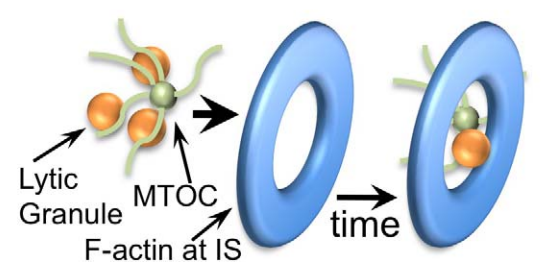
\includegraphics[width=\textwidth]{../figures/chapter1/actinclearance.png}
	\caption{Canonical model of actin clearance as a necessary condition for lytic granule secretion}
	\caption*{Model of central actin clearing for MTOC polarization and lytic granule fusion. Upon TCR activation, MTOC polarizes towards the immune synapse with the assistance of the motor protein dynein, bringing lytic granules towards the IS and docking them in preparation for degranulation. The actin meshwork clears from the center of the IS, forming a mature dSMAC actin-ring (as well as the associated pSMAC and cSMAC) and exposing available synaptic membrane for degranulation. This figure is adapted from \cite{Rak2011}.}
	\label{fig:actinclearance}
\end{figure}

Newer, more recent models of degranulation highlight the need for transient actin polymerization at the site of degranulation to potentiate the pore forming effects of perforin \cite{Tamzalit2018}. This is related to T cell mechanical force exertion against the target, which significantly amplifies T cell effector function \cite{Tamzalit2018}.

\section{T cell mechanical force exertion}
Immune cell-immune cell interactions are typically described as a series of interrelated biochemical receptor-ligand signaling processes (and this introduction has done the same). While this characterization is not incorrect, it ignores the mechanical dimension of immune cell interactions, which have been identified as a significant hubs of cellular decision making. Immune cells have been demonstrated to have a number of biophysical sensing functions, including cancer cell surveillance and immune cell function and cytotoxicity. 

The IS is a physically dynamic structure that exerts mechanical force \cite{Ritter2015, Bashour2014}. Naïve T cells exert mechanical force on polydimethylsiloxane (PDMS) pillars coated with activating proteins, as observed via traction force microscopy \cite{Bashour2014}. It is reasonable to think that T cells have evolved mechanisms to use this force information as a method of sensing the mechanical properties of surfaces that they come in to contact with. This hypothesis is supported by the finding that T cells are more strongly activated on stiffer PDMS surfaces and polyacrylamide gels, rather than softer, as measured by cytokine production and proliferation \cite{Connor2012}. Evidently, avenues of mechanical communication inform the T cell's actions, and vice-versa.

Recent studies demonstrate that the actin-rich structures formed during T cell adhesion and degranulation are actually involved in boosting the lytic activity of perforin by dynamically applying mechanical force against the target cell \cite{Basu2016, Tamzalit2018} and sensitizing the target cell to perforin insertion, which must overcome the hydrophobic interior of the plasma membrane in order to pierce the target cell plasma membrane and trigger cell lysis (see Figure \ref{fig:mechforce}). This phenomenon is an example of \textit{mechanopotentiation}, or the boosting of biochemical functions through mechanical means. This theme is extensively explored throughout this thesis in Chapters \ref{chap:chapter2} and \ref{chap:chapter3}.

\begin{figure}[htbp]
	\centering
	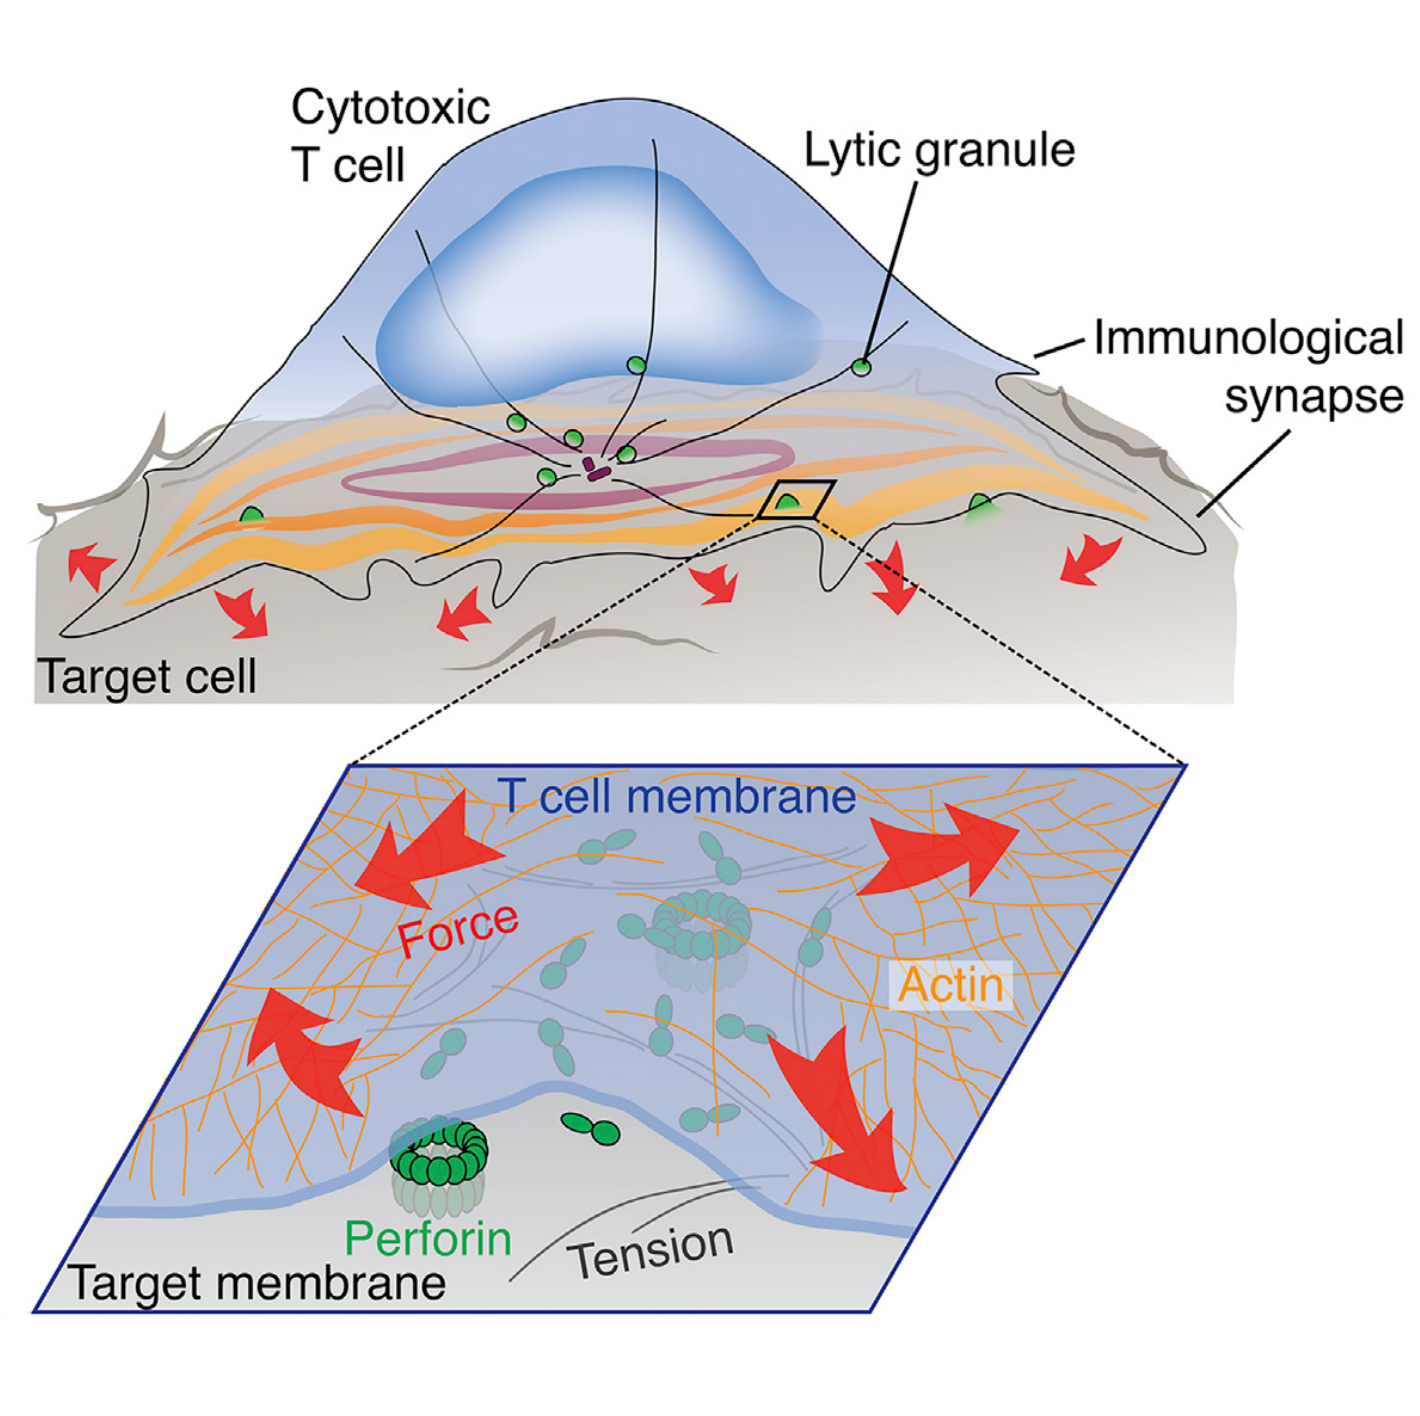
\includegraphics[width=0.8\columnwidth]{../figures/chapter1/mechforce.png}
	\caption{T cells exert mechanical force against target cells}
	\caption*{Illustration of T cell force exertion against the target cell. T cells use biophysical force (via cytoskeletal proteins such as actin) in concert with biochemical signaling axes to optimize their own activation and cytotoxic programming. This force focuses the secretion of lytic granules and the pore-forming effect of perforin. This figure is adapted from \cite{Rak2011}.}
	\label{fig:mechforce}
\end{figure}

We can also look more closely at force application across the immune synapse, at a molecular scale. The exertion of cellular force against a resisting surface occurs via not only through general macroscale membrane-membrane interactions, but also through specific receptor-ligand interactions. Typically, the resistance through receptor-ligand interaction amplifies T cell signaling and function \cite{Huse}. Recent work has demonstrated that the TCR uses mechanical force to both enhance pre-existing TCR-amino acid contacts in a TCR-pMHC context and trigger new amino acid interactions that resist bond dissociation over force, the categorical definition of a catch bond \cite{Wu2019}. The lifetime of TCR-MHC force not only depends on the presence of peptide loaded onto MHC, but also the specific sequence of the peptide \cite{Liu2014}. This implies that T cells are capable of mechanically discerning specific peptide sequence, although the full details of such a mechanism have not yet been identified. Additionally, the lifetime of the resisting TCR-pMHC interaction affects TCR activation on a graded scale (i.e. not biphasic), independently of the peptide in question. This was shown in a study of increased TCR-pMHC lifetime, in which longer TCR-pMHC resisting interactions induced substantially higher levels of calcium flux, as opposed to the same peptide under lower force \cite{Liu2014}. Some work on TCR-$\zeta$ chain opening suggests that TCR clustering induces conformational chains in order to expose phosphorylation sites in its ITAM domains, possibly hinting at a mechanically-based explanation for TCR signal amplification \cite{Aivazian2000}. In totality, current studies point to a possible TCR activation model in which TCR-transduced force serves to lengthen the bond lifetime of the TCR and induce critical membrane proximal signaling events, as described in section \ref{TCR activation and downstream signaling}. 

\begin{figure}[htbp]
	\centering
	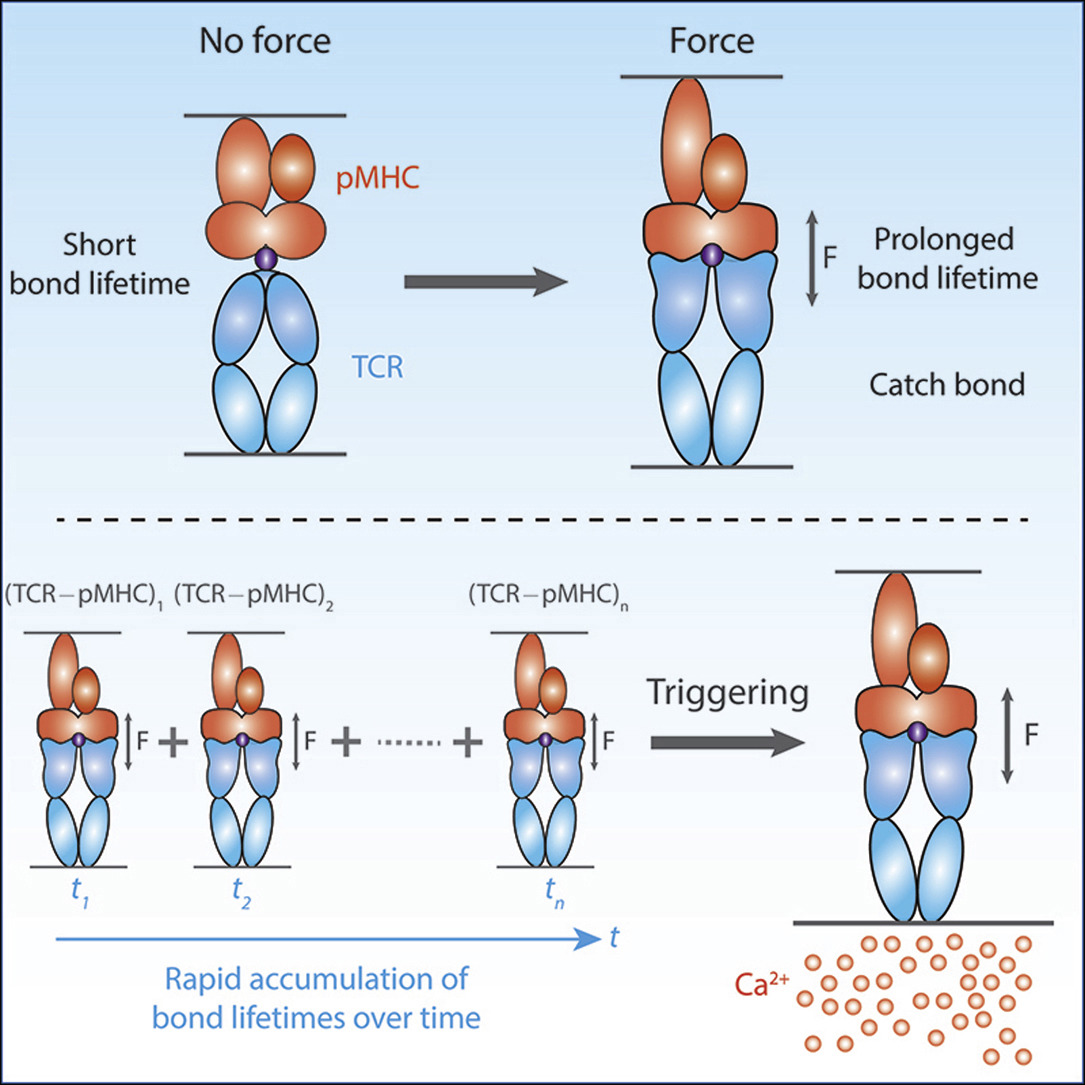
\includegraphics[width=0.8\columnwidth]{../figures/chapter1/tcrcatchbond.jpg}
	\caption{Mechanosensitive receptors of the immune synapse}
	\caption*{An illustration of the principle of mechanosensitive receptors. The lifetime of a receptor-ligand interaction in response to applied force across the bond can either significantly increase the lifetime of the bond (a catch bond) or rapidly decrease (slip bond). The TCR is an example of a mechanosensitive receptor - it demonstrates catch bond behavior with applied force. If a sufficient accumulation of signaling bonds accrue (here, the TCR) then TCR activation is triggered (e.g. flux of $Ca^{2+}$ ions, see \ref{TCR activation and downstream signaling}) and highly potentiated by the increased avidity and number of active TCR-pMHC bonds. This figure is adapted from \cite{Liu2014}.}
	\label{fig:tcrcatchbond}
\end{figure}

Furthermore, the TCR-pMHC interaction actually functions as a catch bond \cite{Liu2014}. A catch bond is a particular type of bond in which application of a force increases the lifetime (to an extent) of the interaction, as opposed to a slip bond, whose lifetime decreases as more force is applied. The TCR's capacity to form a catch bond plays a critical mediating role in the TCR's ability to discriminate between high and low affinity agonists \cite{Liu2014}, as well as in responding differentially between them (i.e. in a graded, not a binary, fashion). A recent report emphasizes the fine-tuning of TCR strength for tumor-specific T cells, in which T cells that received either too high or too low of a signal strength both upregulated inhibitory receptors (such as PD-1) and failed to improve tumor clearance \cite{Shakiba2021}, suggesting a molecular convergence. However, while $signal^{hi}$ tumor-specific T cells lost effector function (suggesting an exhausted state), $signal_{low}$ tumor-specific T cells achieved a functionally inert state, defying expectations of molecular convergence \cite{Shakiba2021}. A complete understanding of the mechanical signaling of T cell-specific receptors remains at large, and will require many years of study to untangle their mechanical activity from their biochemical activity, which remains ever the challenge in mechanobiology. Together these studies demonstrate the important role of mechanobiology in T cell activation and signaling.

Other receptors are also mechanosensitive, including ion channels, G-protein coupled receptors (GPCRs), and integrins \cite{Moroni, Iliff2018, Sun2016}. Integrins are of particular interest to this thesis - see subsection \ref{Integrin biology and mechanotransduction} for further details. Further research is needed to understand the precise role of surface tension on T cell activation. Yet, these studies are intriguing and support the concept that signaling and cell biology are not merely biochemical reactions. These observations show that mechanical properties of biology are important factors that have been largely overlooked in immunology until recently. 

\section{Thesis Aims}
The successful development of immune cell therapies thus far has been dependent on a deeper understanding of basic T cell effector function, and will continue to be. To this end, this thesis is chiefly focused on a molecular approach to studying the mechanotransduction of T cell effector function and the dynamic relationships between its biophysical and biochemical dimensions. The results of this study are broken across two chapters, whose contents are summarized below.

While it was known that the CTLs use physical force to amplify the pore-forming effects of perforin and resulting positive correlation between force exertion and target cell death, it was unclear what cellular structures T cells form in order to actualize this force against the target cell membrane and manipulate this relationship. It was also unclear what proteins or molecules were involved in this membrane perturbation/distortion process. Chapter 2 of this thesis will address the results of the experiments testing these outstanding questions through the use of genetic perturbations against the actin nucleation promoting factors (NPFs) Wiskott–Aldrich Syndrome protein (WASP) and WAVE2 (WASP-verprolin homolog 2) that directly affected T cell force exertion, and studying their resulting cytotoxic capabilities and dynamics via co-culture assays and imaging.

Another outstanding question arose from the observation that T cells degranulate specifically near areas of synaptic force exertion. While this dovetails with the observation that force exertion amplifies the pore-forming effects of perforin (as discussed in the Introduction and Chapter \ref{chap:chapter2}), it was unknown what types of forces or interactions coordinated these two phenomena of degranulation and synaptic force exertion so that they could be unified in space and time. It was also unknown what force-sensitive molecules could be mediating this intercellular communication. Chapter \ref{chap:chapter3} addresses the study conducted to address these questions, which also used pharmacological and genetic perturbations against integrins (primarily lymphocyte function-associated antigen 1, or LFA-1) on T cells in order to modify the force output of these T cells and change their degranulation and cytotoxic behavior as observed through co-culture assays and imaging experiments. A discussion of the implications of the results of Chapters \ref{chap:chapter2} and \ref{chap:chapter3} and possible future directions can be found in the Chapter \ref{chap:discussion}. Altogether, this thesis aims to clarify the specifics of the T cell killing event (encompassing T cell force exertion and degranulation) in order to better inform future T cell studies and therapy design. 
